\documentclass[12pt,a4paper]{article}
\usepackage[utf8]{inputenc}
\usepackage[spanish]{babel}
\usepackage{graphicx}
\usepackage{hyperref}
\usepackage{xcolor}
\usepackage{listings}

\title{Arquitectura y API REST - Documentación Técnica}
\author{TUS DATOS AQUÍ}
\date{FECHA}

\begin{document}

\maketitle
\tableofcontents
\newpage

\section{Arquitectura de Sistemas}
El proyecto \textbf{Catastro Metropolitano} se basa en una arquitectura desacoplada orientada a microservicios, diseñada para alta disponibilidad y sincronización en tiempo real.

\begin{itemize}
    \item \textbf{Frontend:} Desarrollado con React 19 y empaquetado con Vite. Utiliza Tailwind CSS v4 para la estilización. Está alojado de manera estática y distribuida globalmente en Cloudflare Pages.
    \item \textbf{Backend:} Desarrollado en Python 3.11 con \textbf{FastAPI 0.136} y Pydantic v2 para validación estricta de esquemas. Alojado en la plataforma Render.
    \item \textbf{Persistencia (Base de Datos):} Supabase (PostgreSQL) usando el cliente oficial de Python. Se garantiza la atomicidad y consistencia de los datos geoespaciales.
\end{itemize}

\section{Modelo de Datos}
La tabla principal en la base de datos se denomina \texttt{mapas} y cuenta con la siguiente estructura:
\begin{itemize}
    \item \texttt{clave} (TEXT PRIMARY KEY): Identificador único del mapa (ej. \texttt{sur-01}).
    \item \texttt{nombre} (TEXT NOT NULL): Nombre legible del mapa.
    \item \texttt{color\_tema} (TEXT): Color hexadecimal asociado al mapa.
    \item \texttt{width} y \texttt{height} (INTEGER): Dimensiones del canvas en píxeles.
    \item \texttt{config} (JSONB): Almacena toda la geometría compleja (trazos, polígonos, capas) en un formato JSON flexible.
\end{itemize}

\section{API REST y Consumo (Swagger UI)}
El Backend expone una interfaz interactiva de documentación generada automáticamente mediante OpenAPI/Swagger, facilitando las pruebas de integración.

\href{https://tecnologia-atkj.onrender.com/api/docs}{Explorar API en Producción (Swagger)}

\begin{figure}[h]
    \centering
    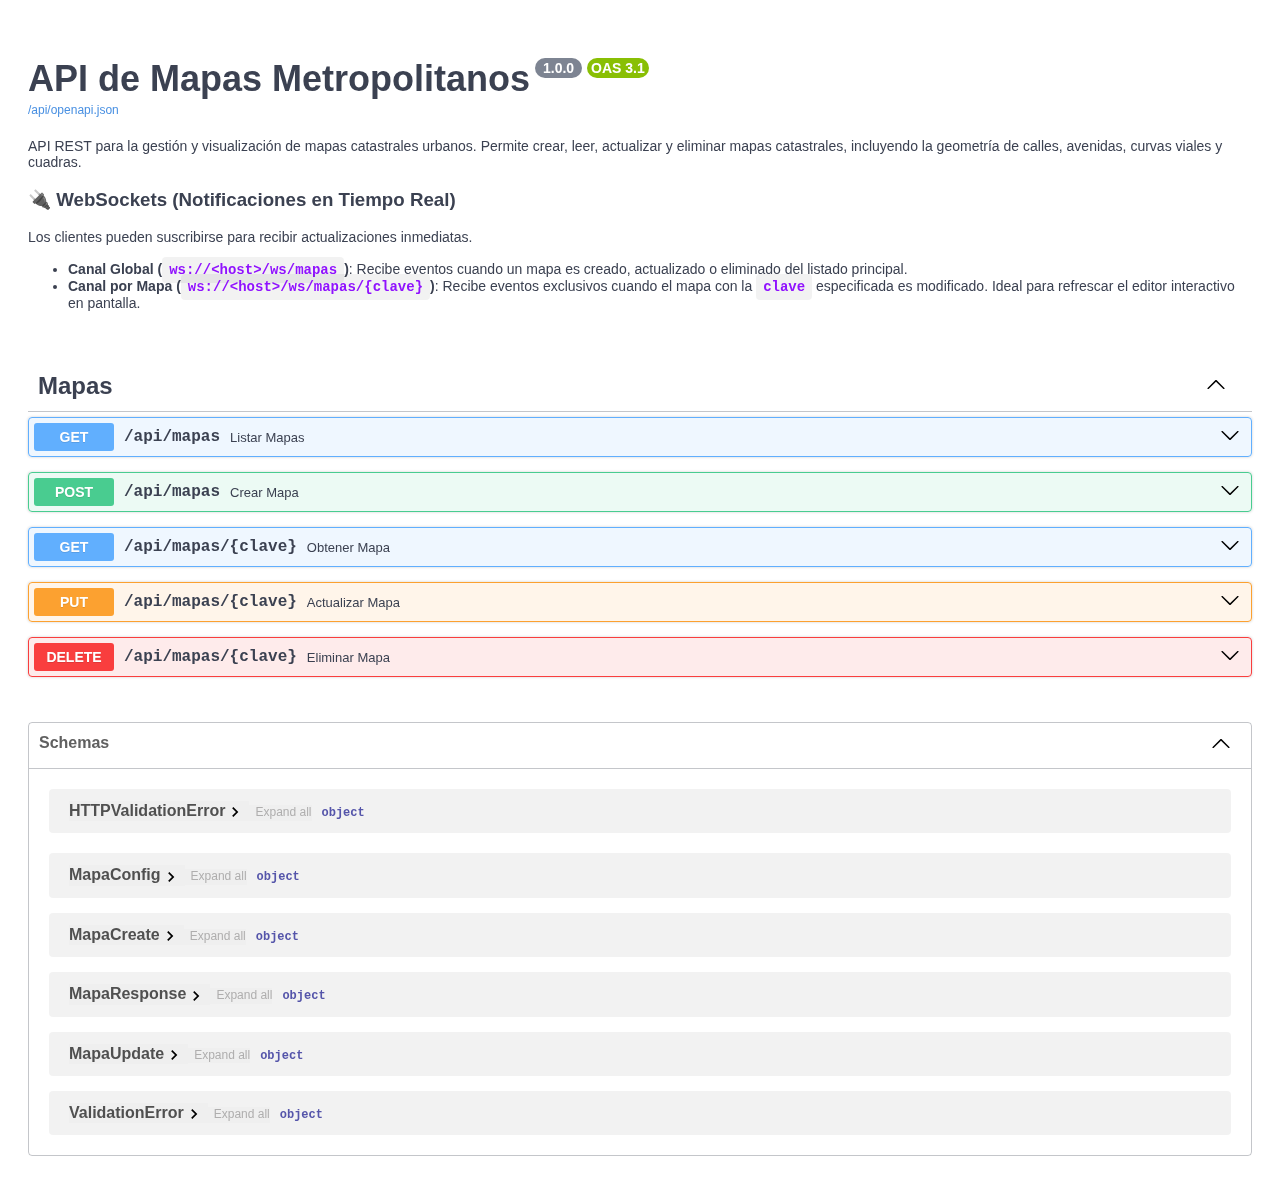
\includegraphics[width=1\textwidth]{../docs_assets/backend_swagger.png}
    \caption{Interfaz interactiva de Swagger UI donde se muestran los endpoints CRUD.}
\end{figure}

\subsection{Operaciones Disponibles:}
\begin{enumerate}
    \item \texttt{GET /api/mapas}: Lista todos los mapas disponibles (solo retorna metadatos básicos para optimizar ancho de banda).
    \item \texttt{POST /api/mapas}: Registra la estructura inicial de un mapa.
    \item \texttt{GET /api/mapas/\{clave\}}: Obtiene el JSON completo, incluyendo la geometría.
    \item \texttt{PUT /api/mapas/\{clave\}}: Actualiza las coordenadas y metadatos.
    \item \texttt{DELETE /api/mapas/\{clave\}}: Elimina un mapa permanentemente de Supabase.
\end{enumerate}

\section{Arquitectura de Tiempo Real (WebSockets)}
Para evitar saturar la base de datos con peticiones constantes (polling), el backend implementa un sistema de notificaciones \textbf{Push} mediante WebSockets de FastAPI.

\subsection{Gestor de Conexiones}
El módulo \texttt{websocket\_manager.py} administra los canales para garantizar el aislamiento de eventos:
\begin{itemize}
    \item \textbf{Canales Específicos} (\texttt{ws://.../ws/mapas/\{clave\}}): Solo transmiten eventos relacionados a ese mapa. Garantiza la seguridad y eficiencia del ancho de banda.
    \item \textbf{Canal Global} (\texttt{ws://.../ws/mapas}): Notifica creación y eliminación de mapas para actualizar listados.
\end{itemize}

\subsection{Estructura del Payload (JSON)}
Cuando ocurre un evento, el servidor emite un JSON con el siguiente formato:
\begin{verbatim}
{
  "event": "mapa:updated",
  "data": {
    "clave": "sur",
    "mapa": { "config": {...} }
  }
}
\end{verbatim}

\subsection{Probador de WebSockets (Tester Local)}
Se ha desarrollado un cliente HTML para probar los sockets de forma local, simulando ser el frontend.

\begin{figure}[h]
    \centering
    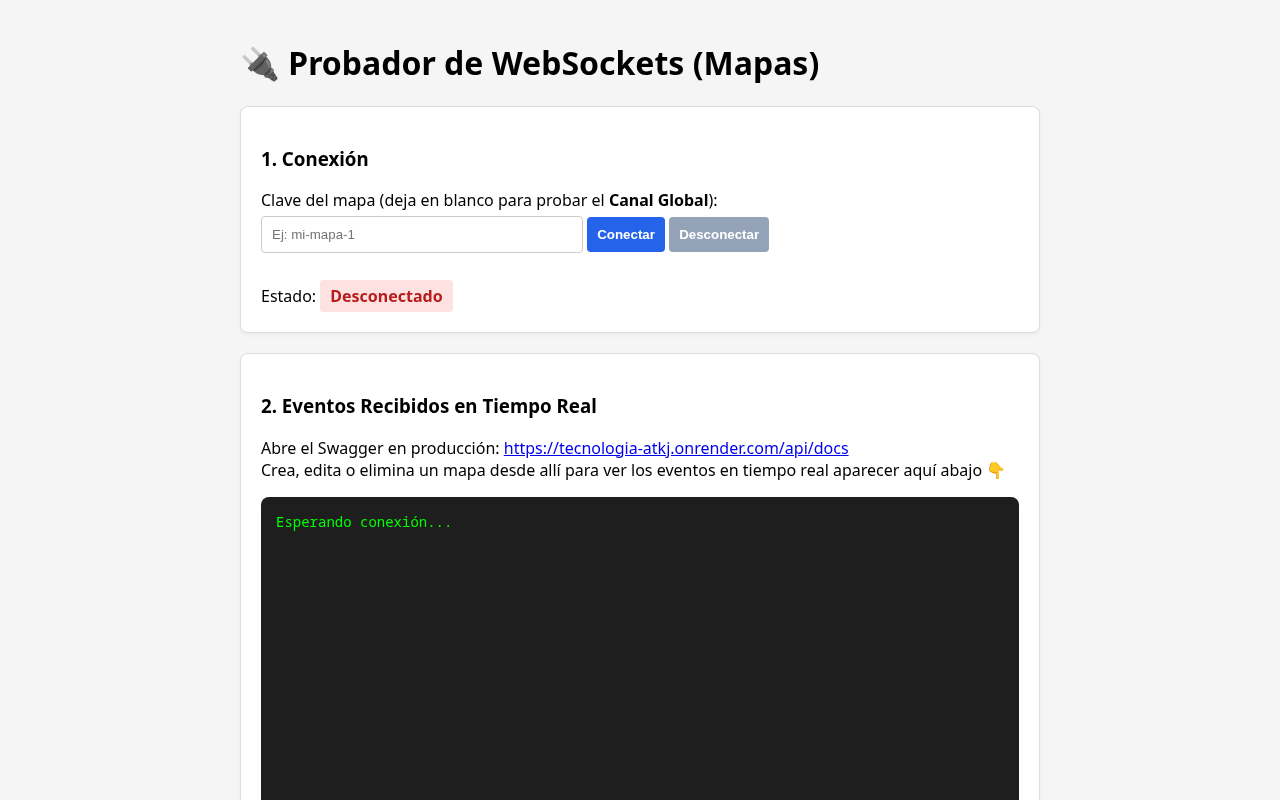
\includegraphics[width=1\textwidth]{../docs_assets/ws_client.png}
    \caption{Consola del probador local mostrando eventos recibidos.}
\end{figure}

\section{Guía de Despliegue Local}
Para ejecutar el proyecto en tu máquina para desarrollo o pruebas:

\subsection{Requisitos Previos}
\begin{itemize}
    \item Python 3.11+
    \item Node.js 20+ con \texttt{pnpm} instalado
\end{itemize}

\subsection{Levantar el Backend (FastAPI)}
Clona el repositorio. Configura un archivo \texttt{.env} en la raíz con \texttt{SUPABASE\_URL} y \texttt{SUPABASE\_KEY}. Luego ejecuta en la terminal:
\begin{verbatim}
pip install -r api/requirements.txt
python -m api.main
\end{verbatim}
Swagger estará disponible en \texttt{http://localhost:8000/api/docs}.

\subsection{Levantar el Frontend (React)}
Abre una nueva terminal, navega a la carpeta \texttt{client/} y ejecuta:
\begin{verbatim}
pnpm install
pnpm run dev
\end{verbatim}
El frontend estará disponible en \texttt{http://localhost:5173}.

\end{document}
